\documentclass{article}
\usepackage{titlesec}
\usepackage[a4paper,margin=2.5cm]{geometry}
\usepackage{lmodern}
\usepackage{amsmath}
\usepackage{float}
\usepackage[dvipdfmx]{graphicx}
\usepackage{caption}
\usepackage{physics}
\usepackage{bm}
\usepackage{amssymb}

\begin{document}

\title{第3回輪講資料 『ロボット制御基礎論』 pp.11-38}
\author{著者: 吉川恒夫 \\ 担当: 脇本 怜奈}
\date{\today}
\maketitle

\section*{概要}

\setcounter{section}{0}
\renewcommand{\thesection}{2.\arabic{section}}

\section{物体の位置と姿勢}
\subsection{物体座標系}
 基準座標系を\(\sum_{A}\), 原点を\(O_A\), 直交する3軸を\(X_A, Y_A, Z_A\)とする。 

\begin{figure}[H]
    \centering
    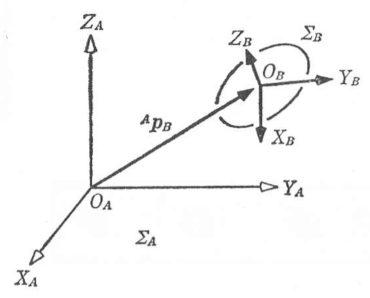
\includegraphics[width=0.3\textwidth]{images/2_1.jpg}
    \caption{図 2.1: 基準座標系と物体座標系}
    \label{fig:2.1}
\end{figure}

\subsection{回転行列}
 回転行列を

\begin{equation}
    ^{A}\vb*{R_B} = 
    \begin{bmatrix}
        ^{A}{\bm{x}_B} & ^{A}{\bm{y}_B} & ^{A}{\bm{z}_B}
    \end{bmatrix}
\end{equation}
と表現する。\(^{A}{\bm{x}_B}\), \(^{A}{\bm{y}_B}\), \(^{A}{\bm{z}_B}\)は互いに直交する単位ベクトルであるので、以下の式(2.3)(2.4)を満たす。
\begin{equation}
    {(^{A}\vb*{R_B})}^T(^{A}\vb*{R_B}) = 
        \bm{I}_3
\end{equation}
\begin{equation}
    {^{A}\vb*{R_B}}^{-1} = 
        {(^{A}\vb*{R_B})}^T
\end{equation}
つまり、回転行列\(^{A}\vb*{R_B}\)は直交行列の性質を持ち、座標変換に用いられる。

\subsection{オイラー角}
\begin{figure}[H]
    \centering
    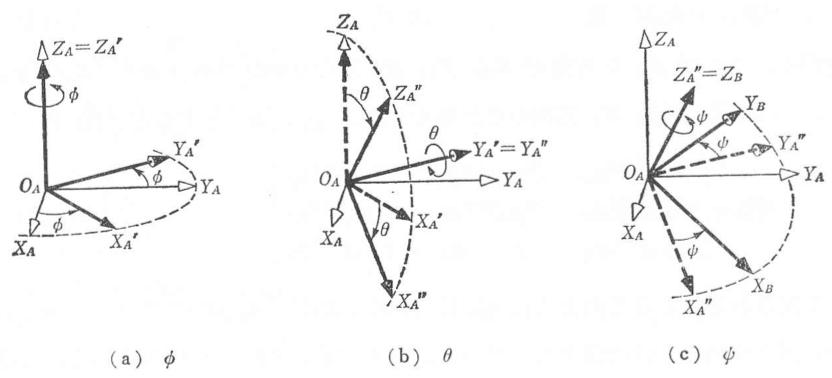
\includegraphics[width=0.7\textwidth]{images/2_4.jpg}
    \caption{図 2.4: オイラー角}
    \label{fig:2.4}
\end{figure}

オイラー角を用いた制御では、図4に示すように物体の姿勢を3つの回転角の組であるオイラー角(\(\phi\), \(\theta\), \(\psi\))で表す。オイラー角が与えられたときの回転行列\(^{A}\vb*{R_B}\)は一意に定まる。\(^{A}\vb*{R_B}\)を式(2.20)に示す。
\begin{equation}
    ^{A}\vb*{R_B} = 
    \begin{bmatrix}
        C_{\phi}C_{\theta}C_{\psi}-S_{\phi}S_{\psi} & C_{\phi}C_{\theta}S_{\psi}-S_{\phi}C_{\psi} & C_{\phi}S_{\theta} \\
        S_{\phi}C_{\theta}C_{\psi}+C_{\phi}S_{\psi} & -S_{\phi}C_{\theta}S_{\psi}+C_{\phi}C_{\psi} & S_{\phi}S_{\theta} \\
        -S_{\theta}C_{\psi} & S_{\theta}S_{\psi} & C_{\theta}
    \end{bmatrix}
\end{equation}

次に、任意の\(^{A}\vb*{R_B}\)から対応するオイラー角を定める。\(^{A}\vb*{R_B}\)を式(2.22)のように定める。
\begin{equation}
    ^{A}\vb*{R_B} = 
    \begin{bmatrix}
        R_{11} & R_{12} & R_{13} \\
        R_{21} & R_{22} & R_{23} \\
        R_{31} & R_{32} & R_{33}
    \end{bmatrix}
\end{equation}

\(\atan2\)を\\
\begin{equation}
    \rm{atan2}(a,b) = \rm{arg}(b+ja)
\end{equation}
とすると、\({R_{13}^2+R_{23}^2} \neq 0\)なら
\begin{equation}
    \theta = \mathrm{atan2} \left(\pm \sqrt{R_{13}^2+R_{23}^2}, R_{33} \right)
\end{equation}
\begin{equation}
    \phi = \mathrm{atan2} \left(\pm R_{23}, \pm R_{13} \right)
\end{equation}
\begin{equation}
    \psi = \mathrm{atan2} \left(\pm R_{32}, \mp R_{31} \right)
\end{equation}

\subsection{ロール・ピッチ・ヨー角}

オイラー角による姿勢表現では\(Z_a^{''}\)軸周りに角度\(\psi\)回転させたが、ロール・ピッチ・ヨー角による姿勢表現では\(X_a^{''}\)軸周りに角度\(\psi\)回転させる。この様子を図(2.6)に示す。

\begin{figure}[H]
    \centering
    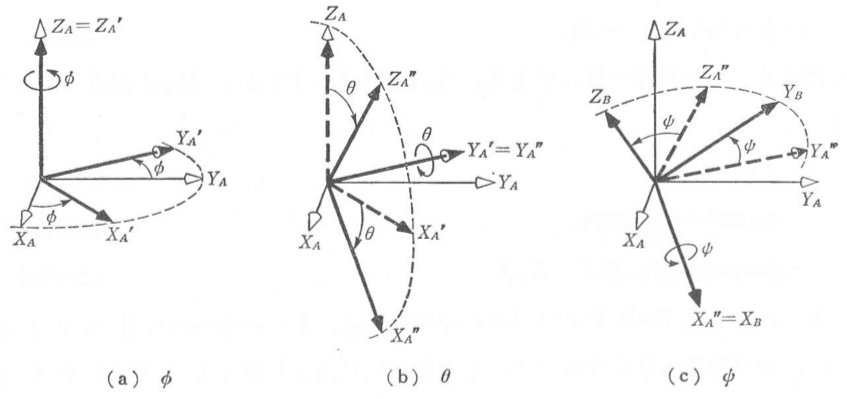
\includegraphics[width=0.7\textwidth]{images/2_6.jpg}
    \caption{図 2.6: ロール・ピッチ・ヨー角}
    \label{fig:2.6}
\end{figure}


\section{座標変換}
\subsection{同次変換}
2つの座標系\(\sum_A\)と\(\sum_B\)について、\(\sum_A\)の座標系の位置を\(^{A} \vb{r}\), \(\sum_B\)の座標系の位置を\(^{B} \vb{r}\), \(\sum_B\)の\(\sum_A\)に対する位置を\(^{A}\vb*{p_B}\)、姿勢の回転行列を\(^{A}\vb*{R_B}\)とすると
\begin{equation}
    \begin{bmatrix}
        ^{A} \vb{r} \\
	1
    \end{bmatrix}
=
    \begin{bmatrix}
       & ^{A}\vb*{R_B} & & ^{A}\vb*{p_B}  \\
	0 & 0 & 0 & 1
    \end{bmatrix}
    \begin{bmatrix}
        ^{B} \vb{r} \\
	1
    \end{bmatrix}
    \triangleq
    ^{A}\vb*{R_B}
    \begin{bmatrix}
        ^{B} \vb{r} \\
	1
    \end{bmatrix}
\end{equation}
と表される。

\section{関節変数と手先位置}
\subsection{一般的関係}
\subsection{リンクパラメータ}
\subsection{リンク座標系}
\subsection{順運動学問題の解}


 



















\end{document}